\documentclass[a4paper,12pt]{article} % добавить leqno в [] для нумерации слева
\usepackage[a4paper,top=1.3cm,bottom=2cm,left=1.5cm,right=1.5cm,marginparwidth=0.75cm]{geometry}
%%% Работа с русским языком
\usepackage{cmap}					% поиск в PDF
\usepackage{mathtext} 				% русские буквы в фомулах
\usepackage[T2A]{fontenc}			% кодировка
\usepackage[utf8]{inputenc}			% кодировка исходного текста
\usepackage[english,russian]{babel}	% локализация и переносы

\usepackage{multirow}
\usepackage{graphicx}
\usepackage{mathtools}
\usepackage{wrapfig}
\usepackage{tabularx}
\usepackage{amssymb}
\usepackage{hyperref}
\usepackage[rgb]{xcolor}
\hypersetup{colorlinks=true,urlcolor=blue}
%% Шрифты
\usepackage{euscript}	 % Шрифт Евклид
\usepackage{amsmath}
\usepackage{mathtools}
%%% Заголовок
\author{Lokhmatov Arseniy}
\title{Лабораторная работа по общей физике}

\date{\today}
\begin{document}
\begin{titlepage}
    \newpage
    \begin{center}
    {\large МОСКОВСКИЙ ФИЗИКО-ТЕХНИЧЕСКИЙ ИНСТИТУТ (НАЦИОНАЛЬНЫЙ ИССЛЕДОВАТЕЛЬСКИЙ УНИВЕРСИТЕТ)}
    \vspace{1cm}

    {\largeФизтех-школа аэрокосмических технологий}
    \vspace{6em}
    \end{center}
    
    \vspace{1.2em}

    \begin{center}
    %\textsc{\textbf{}}
    \Large Лабораторная работа №4.5.1 \\
    Гелий-неоновый лазер
    \linebreak
    \end{center}
    
    \vspace{11em}
    
    \begin{flushright}
                       {\large Работу выполнил\\
                       Лохматов Арсений Игоревич\\
                       Козярский Алексей Сергеевич\\
                       Б03-303 }
    \end{flushright}

    \vspace{\fill}

    \begin{center}
        
\includegraphics[width=0.2\linewidth]{dasr.png}
    \end{center}

    \begin{center}
    Долгопрудный, 2025
    \end{center}

    \end{titlepage}

\section{Теоретическая часть}


\paragraph{Цель работы: } изучение основный принципов работы газового лазера и свойств лазерного излучения.

\paragraph{В работе используются: } юстировочный лазер, гелий-неоновая трубка, компьютер со звуковой картой, модулятор, фотодиоды, зеркала, поляроид.

\paragraph{} Главными элементами практически любого лазера являются два параллельных друг другу зеркала и расположенная между ними среда, усиливающая свет. Параллельные зеркала образуют оптический резонатор и осуществляют положительную обратную связь, превращающую усилитель в генератор. В такой системе самопроизвольно из шума возникает излучение, распространяющееся от одного зеркала к другому и обратно перпендикулярно поверхности зеркал. Любое излучение, распространяющееся под значительным углом к этому направлению, при последовательных отражениях быстро покидает резонатор, не успевая заметно усилиться. Поэтому формируется пучок излучения высокой направленности. Для вывода части излучения наружу одно из зеркал обычно делается полупрозрачным.

Ключевым условием работы лазера является наличие усиливающей среды. Усиление света основано на явлении вынужденного излучения, которое является обратным поглощению света. Как известно из опыта, при поглощении электромагнитного излучения веществом атомы или молекулы, находящиеся на каком-либо энергетическом уровне, переходят на более высокий свободный уровень, поглощая один квант (фотон) излучения. Поглощение возникает только в том случае, если энергия фотона совпадает с разницей энергий между этими уровнями. Явление вынужденного излучения заключается в том, что если атом находится на возбуждённом уровне, то под действием электромагнитного поля происходит обратный переход с возбуждённого уровня на более низкий уровень с излучением кванта света. При этом для конкретной пары уровней вероятность перехода сверху вниз совпадает с вероятностью перехода снизу вверх при одинаковой интенсивности вынуждающего излучения. Следует отметить, что находящиеся на возбуждённом уровне атомы или молекулы могут независимо от наличия вынуждающего поля самопроизвольно переходить на более низкий энергетический уровень, излучая фотон в произвольном направлении. Это явление называется спонтанным излучением, оно присутствует в любой лазерной среде и затрудняет работу лазера, уменьшая заселенность верхнего рабочего уровня. В то же время оно выполняет и полезную функцию, являясь $"\text{затравкой}"$ для формирования направленного пучка лазерного излучения.

Поскольку для любых двух энергетических уровней вероятность вынужденного перехода снизу вверх и сверху вниз одинакова, то усиление может возникнуть только если на верхнем уровне окажется больше атомов, чем на нижнем. Такая ситуация называется инверсной заселенностью. Инверсной населённости можно достичь только в неравновесном состоянии, например, путём оптического заселения верхнего рабочего уровня через дополнительный ещё более высокий уровень. Поэтому все лазеры с оптической накачкой работают, как минимум, по трёхуровневой схеме. 

Ниже будут описаны основные закономерности и свойства лазерного излучения на примере гелий-неонового лазера, при этом большинство выводов справедливо и для других типов лазеров при учёте их конкретных свойств.

\begin{figure}[h]
\begin{center}
    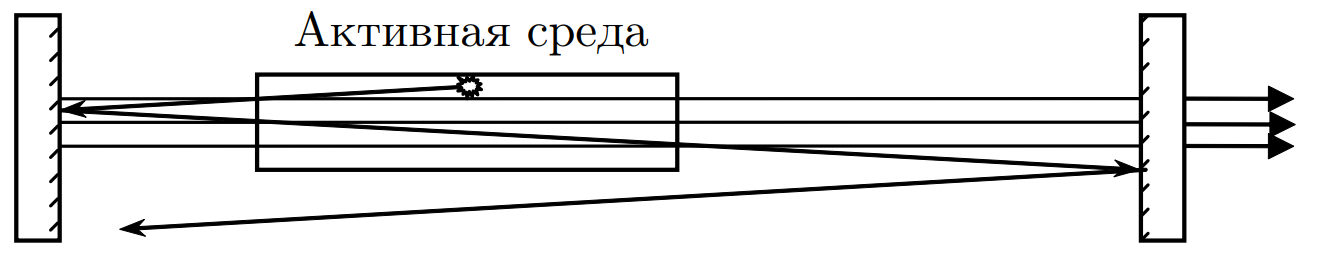
\includegraphics[width=12cm]{image1.png}
\end{center}
    \caption{Схема лазера}
    \label{img1}
\end{figure}

\paragraph{Условное достижение порога генерации.} Выведем пороговое условие генерации в лазере. Для этого рассмотрим простейшую схему лазера, состоящего из плоско-параллельного резонатора (рисунок $\ref{img1}$), образованного двумя зеркалами, имеющими коэффициенты отражения $R_1$ и $R_2$, активной среды, имеющей усиление $G$ на один проход и дополнительных элементов, размещённых внутри резонатора с общим пропусканием $T$ за один проход. Этими дополнительными элементами могут быть, например, стеклянные окна лазерной трубки, вносящие потери излучения за счёт отражения от поверхностей. Возможны и другие виды потерь, приводящие к уменьшению пропускания, например, за счёт дифракционного расплывания пучка. Дифракционные потери становятся существенными при малых поперечных размерах зеркал или активного элемента, сравнимых с размером одной зоны Френеля для расстояния, равного длине резонатора, то есть $r_{las}\approx\sqrt{\lambda L}$. Для получения генерации необходимо, чтобы усиление было достаточным для компенсации всех потерь при полном обходе резонатора.

\[ R_1R_2T^2G^2\geq1\text{ } \Rightarrow\text{ } G\geq \frac{1}{T\sqrt{R_1R_2}}. \]

В непрерывных лазерах в установившемся режиме потери излучения в точности компенсируются усилением и усиление активного элемента за один проход равно

\[ G=\frac{1}{T\sqrt{R_1R_2}}. \]

\paragraph{Гелий-ноновый лазер.} Рассмотрим механизм возникновения усиления в рабочей среде гелий-неонового лазера. Лазерная трубка заполняется смесью гелия и неона, в
которой довольно легко возбудить постоянный электрический разряд. Рабочим лазерным веществом является неон. Гелий используется для избирательного заселения верхнего рабочего уровня неона. Атомы гелия возбуждаются при столкновениях с разогнанными в электрическом поле разряда электронами. Передача энергии от возбуждённых атомов гелия к атомам неона осуществляется при столкновениях между ними. Известно, что наиболее эффективно передача энергии от атома к атому происходит в резонансном случае, то есть когда энергии уровней, между которыми происходит переход, близки. Однако, во всех промышленных лазерах на неоне для увеличения эффективности накачки используют селективное заселение верхних лазерных уровней атомами гелия, поэтому
и называются гелий-неоновыми. Следует отметить, что для поддержания инверсной населённости при работе непрерывного лазера необходимо не только заселение верхнего лазерного уровня, но и быстрое опустошение нижнего. В гелий-неоновом лазере это происходит при соударении атомов неона, находящихся на нижнем лазерном уровне, со стенками лазерной трубки, при этом атомы передают энергию стенкам и сбрасываются ещё ниже, в основное состояние. Недостаточно быстрое опустошение нижнего лазерного уровня в гелий-неоновых лазерах ограничивает и предельный коэффициент усиления, достигаемый при некотором оптимальном разрядном токе. При дальнейшем увеличении тока нижний уровень не успевает опустошаться и эффективность генерации падает. Обычно достигается усиление всего $1–3\%$ за один проход, то есть $G=1.01 – 1.03$. При таком малом усилении генерация вынужденного излучения может быть получена только если окна лазерной трубки либо очень хорошо просветлены, либо расположены под углом Брюстера к оси резонатора, при этом для одной из поляризаций потери на отражение от окошек исчезают. Отражение зеркал резонатора должно быть очень высоким, поэтому используются специальные зеркала, в которых на стеклянную подложку нанесены (обычно напылением) чередующиеся слои диэлектриков с сильно различающимися показателями преломления. Толщины слоёв подобраны таким образом, чтобы все волны, отражённые от границ разделов слоёв, на выходе складывались в фазе.

\begin{figure}[h]
\begin{center}
    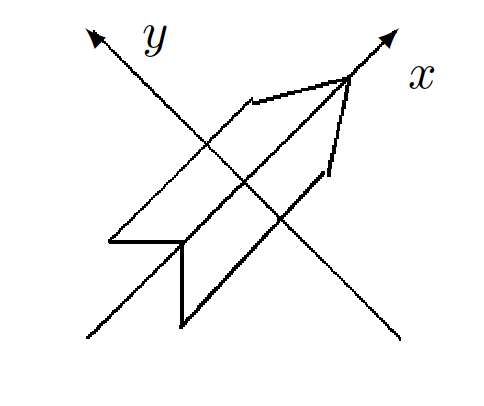
\includegraphics[width=16cm]{image3.png}
\end{center}
    \caption{Устройство гелий-неонового лазера}
    \label{img3}
\end{figure}

Типичная конструкция гелий-неонового лазера изображена на рисунке $\ref{img3}$. Обычно используется сферический или полусферический резонатор, предъявляющий гораздо более мягкие требования к точности юстировки зеркал и обеспечивающий повышенную механическую стабильность по сравнению с плоским резонатором.

\paragraph{Ширина спектра излучения гелий-неонового лазера.} Время жизни верхнего лазерного уровня составляет $10^{-8}\text{ с}$. Из принципа неопределённости $\Delta\nu\cdot\tau\geq1$ можно получить оценку ширины линии $\Delta\nu\geq10^8\text{ Гц}$. Реальная ширина спектра генерации обычного гелий-неонового лазера на порядок больше. Основной механизм уширения -- эффект Доплера. В лазерной трубке атомы неона участвуют в хаотическом тепловом движении. Частота излучения движущегося источника сдвинута относительно неподвижного источника

\[ \Delta\nu=\nu\frac{v}{c}cos{\theta}. \]

Поскольку при хаотическом движении $cos{\theta}$ принимает значения от $1$ до $-1$, то уширение линии приблизительно составляет

\[ \Delta\nu\approx2\nu\cdot\frac{v_{\text{ср}}}{c}=2\nu\sqrt{\frac{8kT}{\pi mc^2}}, \]
где $v_{\text{ср}}$ -- средняя скорость молекул. Точный вывод на основе распределения Максвелла приводит к формуле для полуширины линии которая даёт значение на $40\%$ меньше, чем полученная нами оценочная формула.

\paragraph{Продольные моды.} Рассмотрим более детально спектральный состав излучения исследуемого лазера. Обычно спектр состоит из нескольких эквидистантных линий, соответствующих различным продольным модам резонатора. Модами называют стационарные типы колебаний электромагнитного поля в резонаторе. Если бы зеркала резонатора были металлическими, то минимальные потери имели бы те типы колебаний, для которых электрическое поле на поверхности зеркал равно нулю. Для этого на длине резонатора должно укладываться целое число полуволн. В этом случае после полного обхода резонатора набег фазы световой волны кратен $2\pi$.

В случае диэлектрических многослойных зеркал это условие не столь очевидно. Рассмотрим простейший резонатор из двух зеркал с коэффициентами отражения $R_1$ и $R_2$ и бесконечно тонкий слой усиливающего вещества внутри резонатора с усилением $G$ за один проход. Примем, что состояние лазера стационарно и мощность спонтанного излучения слабо зависит от частоты (ширина линии усиления лазерной среды много шире межмодового расстояния, что выполняется для гелий-неонового лазера). Чтобы найти мощность излучения внутри резонатора в каком-либо месте, например, на внутренней поверхности выходного зеркала, нужно просуммировать после последовательных проходов комплексные амплитуды волн, излучаемых лазерной средой в левую сторону, умножить на комплексносопряжённую величину, потом проделать то же для волн, излучаемых вправую сторону и затем сложить. Получается формула

\[ P(\omega)\sim\frac{1}{(1-\sqrt{R}G)^2+4\sqrt{R}Gsin^2{\frac{\varphi}{2}}}, \]
где $R=R_1R_2$, а $\varphi$ -- набег фазы при полном обходе резонатора. Эта функция имеет резкие максимумы при $\varphi=2\pi n$, поскольку в стационарном состоянии $\sqrt{R}G\approx1$.

Таким образом, для многослойных диэлектрических зеркал  набег фазы при полном обходе резонатора должен быть кратен $2\pi$. Значит, на длине резонатора должно укладываться целое число полуволн, только в случае многослойных зеркал длина резонатора не обязательно совпадает с геометрическим расстоянием между поверхностями зеркал, а определяется фазой, с которой эти зеркала отражают световую волну. Это различие сравнимо с длиной волны, то есть много меньше обычных длин резонатора, поэтому расстояние между продольными модами получается практически таким же,
как в случае металлических зеркал.

\paragraph{Поперечные моды.} 

\begin{wrapfigure}{r}{0.45\linewidth}
    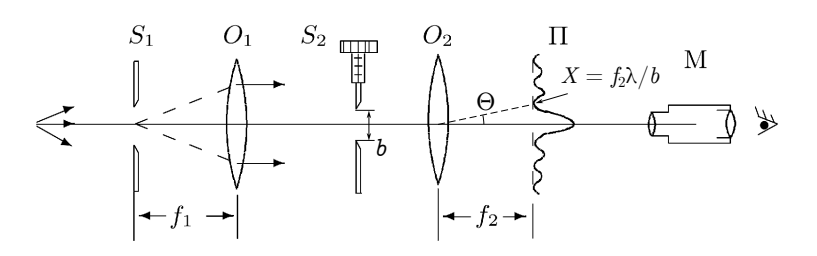
\includegraphics[width=\linewidth]{image4.png}
    \caption{Направления распространения мод с разными поперечными индексами}
    \label{img4}
\end{wrapfigure}

Анализ углового распределения лазерного излучения удобнее проводить для случая квадратных зеркал резонатора, причём поперечный размер активной среды превышает ширину $D$ зеркал, то есть лазерный пучок ограничивается зеркалами. Излучение, распространяющееся под небольшим углом к оси резонатора может испытать достаточное число проходов, чтобы заметно усилиться и присутствовать в выходном излучении. Однако, допустимые углы должны удовлетворять определённым соотношениям, вытекающим из свойств резонаторов. Простейшая теория лазерных резонаторов Шавлова и Таунса основана на сходстве открытых (без боковых стенок) резонаторов с закрытыми. Однако, основные
результаты этой теории можно получить и без аналогий с закрытыми резонаторами. В процессе усиления излучения от спонтанных шумов до стационарного уровня «выживают» только моды, имеющие минимальные потери на дифракцию. Для этого интенсивность излучения на краях зеркал должна быть минимальной, в идеале равной нулю. Если какая-либо мода содержит две волны, распространяющиеся под малыми углами $\pm\theta$ к оси резонатора, то при сложении этих волн на зеркале создаётся интерференционная картина с периодом $\frac{\lambda}{2}\theta$. Для обращения интенсивности в ноль на краях зеркала необходимо, чтобы на ширине зеркала $D$ укладывалось целое число периодов, поэтому $\theta=\pm m\frac{\lambda}{2}D$. Такое же условие должно выполняться по второй
координате в плоскости зеркала $\theta=\pm p\frac{\lambda}{2}D$. Здесь $m$ и $p$ -- целые числа. Результирующий угол равен

\[ \theta=\pm\sqrt{m^2+p^2}\frac{\lambda}{2}D\approx\sqrt{m^2+p^2}\frac{\theta_{\text{дифр}}}{2}, \]
где $\theta_{\text{дифр}}\approx\lambda/D$ -- дифракционная расходимость лазерного пучка с поперечным размером $D$.

Для классификации лазерных мод применяют обозначение $TEM_{mpq}$, имея в виду, что электрическое и магнитное поля $E$ и $H$ перпендикулярны направлению распространения пучка. Типы колебаний с различающимися значениями поперечных индексов $m$ или $p$ называются поперечными модами, с различными $q$ — продольными. Фактически значение поперечного индекса даёт число нулей в распределении интенсивности излучения по соответствующей координате на поверхности зеркала, не считая нулей на краях. Значение продольного индекса $q$ равно числу полуволн, укладывающихся на длине резонатора.

На рисунке $\ref{img4}$ и $\ref{img5}$ схематически показаны направления распространения разных поперечных мод и распределение интенсивности излучения на зеркале по одной из поперечных координат.

Найдём сдвиг частоты поперечных мод относительно чисто продольных. Для моды $TEM_{mpq}$, распространяющейся под углом $\theta$ к оси резонатора составляющая волнового вектора по оси резонатора равна $k_z=q\pi/L$, где $L$ -- длина резонатора. Составляющая в плоскости зеркал равна $k_{x,y}=k\sin{\theta}\approx k_z\theta$. Учитывая, что $m,p\leq q, \text{ }\theta\ll1, \text{ }\omega=kc$, получаем для угла $\theta$

\[ \omega_{mpq}\approx\omega_{00q}\Big[1+\frac{1}{8}(m^2+p^2)\frac{\lambda^2}{D^2}\Big]. \]

\begin{wrapfigure}{r}{0.55\linewidth}
    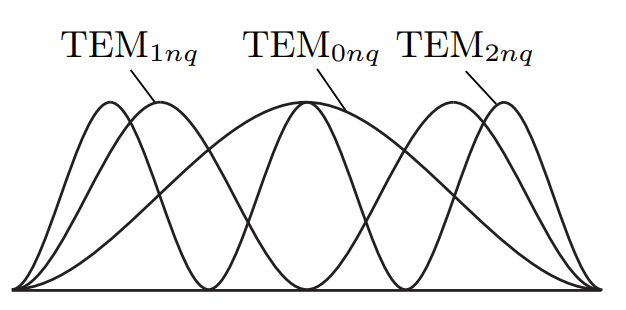
\includegraphics[width=\linewidth]{image5.png}
    \caption{Распределение интенсивности лазерного излучения на зеркале резонатора по одной из поперечных координат для трёх низших поперечных мод}
    \label{img5}
\end{wrapfigure}

Полезно оценить разницу частот чисто продольной моды и поперечной моды с таким же продольным индексом и сравнить её с межмодовым расстоянием для продольных мод. Учитывая, что $\omega_{00q}\approx2\pi c/\lambda$, где $\lambda$ -- средняя длина волны лазерного излучения, получим

\[ \frac{\omega_{mpq}-\omega_{00q}}{\omega_{00q+1}-\omega_{00q}}\approx(m^2+p^2)\frac{\lambda L/4}{D^2}. \]

Обычно размер лазерного пучка ограничивается не зеркалами, а другими элементами, например, лазерной трубкой, но это обстоятельство мало сказывается на характере распределения поля в сечении пучка и модовой структуре выходного излучения. Кроме того, обычно зеркала и другие элементы не квадратные, а круглые. Это должно приводить к цилиндрической симметрии распределения поля по площади пучка и по углам. Однако, из-за неконтролируемых дефектов зеркал, пыли и неточностей юстировки обычно происходит самопроизвольное выделение преимущественного поперечного направления и распределение интенсивности по сечению выходного пучка чаще всего напоминает прямоугольный вариант, принимая иногда разнообразные формы в зависимости от качества юстировки зеркал резонатора.

\begin{wrapfigure}{r}{0.45\linewidth}
    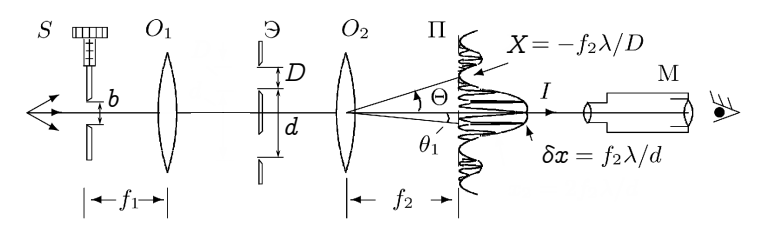
\includegraphics[width=\linewidth]{image6.png}
    \caption{Примерный вид спектра излучения гелий-неонового лазера}
    \label{img6}
\end{wrapfigure}

Типичный спектр излучения гелий-неонового лазера схематически изображён на рисунке $\ref{img6}$. Для наглядности пропорции искажены: в действительности поперечные моды ближе к соответствующей чисто продольной моде, а ширина спектра отдельных мод меньше, чем изображено на рисунке. Соотношение между амплитудами различных мод носит случайный характер и меняется со временем.

\paragraph{Когерентность лазерного излучения.} Выходящее из лазера излучение практически повторяется с периодом, равным времени обхода светом резонатора. Однако, с каждым обходом такие характеристики излучения, как форма огибающей и фаза всё-таки слегка изменяются, поскольку часть излучения постоянно покидает резонатор через выходное зеркало и на его место приходит та часть усиленного спонтанного излучения, которая попадает в полосу усиления лазерной среды и совпадает по частотному и пространственному спектру со спектром мод резонатора. При этом фаза "подмешанного"  спонтанного излучения имеет случайное значение.

Оценим минимальную задержку, при которой падает контраст интерференционной картины. Если лазер генерирует $m$ продольных мод с волновыми векторами от $\pi q/L$ до $\pi(q+m-1)/L$, то при разности фаз, равной $\pi$ для крайних мод, максимумы одной крайней моды попадают на минимумы другой и контраст начинает заметно падать. Это произойдёт при геометрической задержке $l=L/(m+1)$, что для типичного гелий-неонового лазера составляет $l\approx10$ см. Оценку можно сделать и из других соображений. Поскольку полная ширина спектра излучения равна расстоянию между крайними модами $\Delta\nu=c(m-1)/2L$, то время, в течении которого когерентность заведомо сохраняется, равно $\tau=1/\Delta\nu$, следовательно $l=c\tau=2L/(m-1).$

\begin{figure}[h]
\begin{center}
    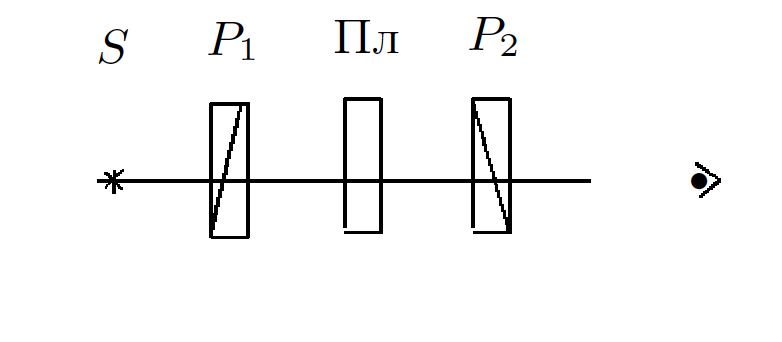
\includegraphics[width=16cm]{image7.png}
\end{center}
    \caption{Схема установки. Штриховыми линиями показано положение зеркал при получении лазерной генерации на исследуемой трубке}
    \label{img7}
\end{figure}

\paragraph{Экспериментальная установка.} Схема экспериментальной установки приведена на рисунке $\ref{img7}$. На оптической скамье расположены: газоразрядная трубка исследуемого $He-Ne$ лазера $\text{ЛГ-75}$ $(1)$, рейтера для крепления юстировочных оправ с зеркалами $(2, 3, 4)$, линза, уменьшающая расходимость юстировочного лазера $(5)$, фотодиод $(6)$, модулятор $(7)$ а также съемный рейтер $(8)$ с отрицательной линзой для наблюдения модовой структуры излучения исследуемого лазера и рейтер $(9)$, в который вставляется либо экран, либо поляроид. Юстировочный лазер $(10)$ и фотодиод
$(11)$ закреплены на столе. Модулятор может быть повёрнут в разные положения: при измерении коэффициента усиления он модулирует пучок, идущий от юстировочного лазера, при измерении поляризации излучения исследуемого лазера он модулирует это излучение, а в остальных случаях он отводится в сторону, чтобы не перекрывать пучки. Юстировочный лазер предназначен для юстировки всех элементов установки и для измерения коэффициента усиления активной среды исследуемого лазера.

\newpage

\section{Практическая часть}

В работе предлагается измерить коэффициент усиления лазера; добиться генерации и изучить модовую структуру излучения в зависимости от настройки зеркал лазера и характер поляризации лазерного луча.

\begin{enumerate}
    \item Включили вилку питания юстировочного лазерав сеть и убедились в наличии лазерного излучения.
    \item Провели юстировку оптической системы. Для удобной юстировки мы сняли выходное зеркало вместе с рейтером, модулятор отвели в сторону, чтобы он не перегораживал пучки. В результате луч юстировочного лазера попадает на полупрозрачное зеркало на оптической скамье, которое напрявляет его на исследуемую трубку. Пятно на экране мы видели с ровными краями, и при малой расстойки вверх-вниз и влево-вправо форма пятна почти не меняется. Значит, устировка проведена хорошо!
    \item Измерение коэффициента усиления производились с помощью компьютера и программы $PhysLab$.
    Фотодиод $(6)$ за полупрозрачным зеркалом следует выставить так, чтобы прошедший через зеркало пучок попадал на приёмную площадку фотодиода. Прошедший исследуемую трубку пучок с помощью заднего зеркала направляется на приёмную площадку фотодиода $(11)$. Включили мотор модулятора и расположили его так, чтобы он прерывал пучок юстировочного лазера до попадания на полупрозрачное зеркало. Выбрали удобные параметры осцилографа в $PhysLab$ и пронаблюдали сигналы с обоих фотодиодов. Мы проделали данную процедуру при нескольких значениях разрядного тока, но коэффициент усиления удалось измерить только на одном! Результаты измерений представлены в таблице $\ref{tab1}$.

    \begin{table}[h]
        \centering
        \begin{tabular}{|c|c|}
        \hline
            \multicolumn{2}{|c|}{$I_0=0\text{ мА}$} \\ \hline
        \hline
    	$N$ & $Eff.Ch.2, \text{ мВ}$ \\ \hline
            1 & 46.412 \\ \hline
            2 & 46.254 \\ \hline
            3 & 45.669 \\ \hline
            4 & 45.978 \\ \hline
            5 & 45.888 \\ \hline
            6 & 45.640 \\ \hline
            7 & 45.914 \\ \hline
            8 & 45.961 \\ \hline
            9 & 45.809 \\ \hline
            10 & 45.955 \\ \hline
            11 & 45.898 \\ \hline
        \end{tabular}
        \begin{tabular}{|c|c|}
        \hline
            \multicolumn{2}{|c|}{$I_1=52\text{ мА}$} \\ \hline
        \hline
    	$N$ & $Eff.Ch.2, \text{ мВ}$ \\ \hline
            1 & 46.724 \\ \hline
            2 & 46.732 \\ \hline
            3 & 46.453 \\ \hline
            4 & 46.376 \\ \hline
            5 & 46.490 \\ \hline
            6 & 46.515 \\ \hline
            7 & 46.492 \\ \hline
            8 & 46.609 \\ \hline
            9 & 46.675 \\ \hline
            10 & 46.590 \\ \hline
            11 & 46.544 \\ \hline
        \end{tabular}
    \caption{Результаты измерений}
    \label{tab1}
    \end{table}

    При обработке результатов мы поделили значения на втором фотодиоде с включённым источником источником и без него, а затем усреднили результат по времени. Получили следующий коэффициент усиления

    \[ k = \overline{\Big(\frac{E_{52}}{E_0}\Big)} = 1.014, \text{ т.е. } 1.4\%. \]

    Также оценим погрешность измерений. Значение со второго фотодиода на осциллографе при выключенном источнике менялось от $45.640\text{ мВ}$ до $46.412\text{ мВ}$, в среднем значение составляло $45.943\text{ мВ}$, то есть относительная погрешность при выключенном источнике тока составляет $\varepsilon=1.1\%$. Значение со второго фотодиода на осциллографе при включенном источнике тока менялось от $46.376\text{ мВ}$ до $46.732\text{ мВ}$, в среднем значение составляло $46.564\text{ мВ}$, то есть относительная погрешность при выключенном источнике тока составляет $\varepsilon=0.4\%$. 
    
    Окончательно, коэффициент усиления активной среды при токе источника $I=52\text{ мА}$ равен

    \begin{center}
       \boxed{k=1.4\%,\text{ } \varepsilon=1.1\%} 
    \end{center}
    
    \item Провели настройку исследуемого лазера для получения генерации. Сначала настроили глухое (заднее сферическое зеркало, выходное зеркало при этом было снято. Пучок, прошедший через трубку, задним зеркалом направляется строго обратно так, чтобы после вторичного прохождения через трубку исследуемого лазера он попал на экран, закреплённый на выходном торце зондирующего лазера. Пятно на этом экране яркое, ровное, без ореолов, и его центр совпадает с центром выходящего пучка зондирующего лазера -- значит настройка точна! Поставили на скамью перед трубкой рейтер с выходным зеркалом, рабочей поверхностью к исследуемому лазеру. Это зеркало было отюстировано так, чтобы отражённый от него луч зондирующего лазера попал в то же самое место, куда попадал пучок, отражённый от сферического заднего зеркала. Включили блок питания и дождались, когда загорелся разряд, появилась генерация.
    \item Изучили поляризацию лазерного луча. Для этого закрепили в рейтере перед выходным зеркалом поляроид. Повернули и настроили фотодиод и модулятор так, чтобы пучок исследуемого лазера хорошо проходил сквозь отверстия модулятора и попадал на фотодиод (6). Юстировочный лазер на время проведения этих измерений выключили. Измерили зависимость интенсивности излучения исследуемого лазера в зависимости от угла поворота поляроида. Для этого поворачивали поляроид на определённый угол, и измеряли значения с фотодиода (6) в течении некоторого времени, затем усредняли его по времени. Результаты измерений представлены в таблице $\ref{tab2}$.

    \begin{table}[h]
        \centering
        \begin{tabular}{|c|c|}
        \hline
    	$\varphi, \circ$ & $Eff.Ch.1, \text{ мВ}$ \\ \hline
            40 & 2.835 \\ \hline
            50 & 3.667 \\ \hline
            60 & 4.417 \\ \hline
            70 & 6.241 \\ \hline
            80 & 7.137 \\ \hline
            90 & 7.328 \\ \hline
            100 & 6.462 \\ \hline
            110 & 5.297 \\ \hline
            120 & 3.795 \\ \hline
            130 & 3.061 \\ \hline
            140 & 2.027 \\ \hline
        \end{tabular}
    \caption{Результаты измерений}
    \label{tab2}
    \end{table}

    Построили график зависимости относительной интенсивности от угла поворота поляроида. Результат представлен на рисунке $\ref{img8}$.

    Немного опишем процесс построения. Мы замерили зависимость интенсивности на фотодиоде при разных направлениях осей поляроида. Интенсивность - это мощность на единичную площадку. Поэтому мы отнормировали наши значения с фотодиода по максимальному и возвели полученное значение в квадрат, таким образом, мы избавились от зависимости от площади фотодиода и возникающего тока на элементе. В итоге, получили относительную интенсивность. На графике не показано, но мы проверили, что при дальнейшем вращении поляроида максимум сменяется минимумом и наоборот. 

    Можно сделать вывод о том, что лазер имеет линейную поляризацию, поскольку интенсивность его меняется при повороте осей поляроида.

    \begin{figure}[h]
    \begin{center}
        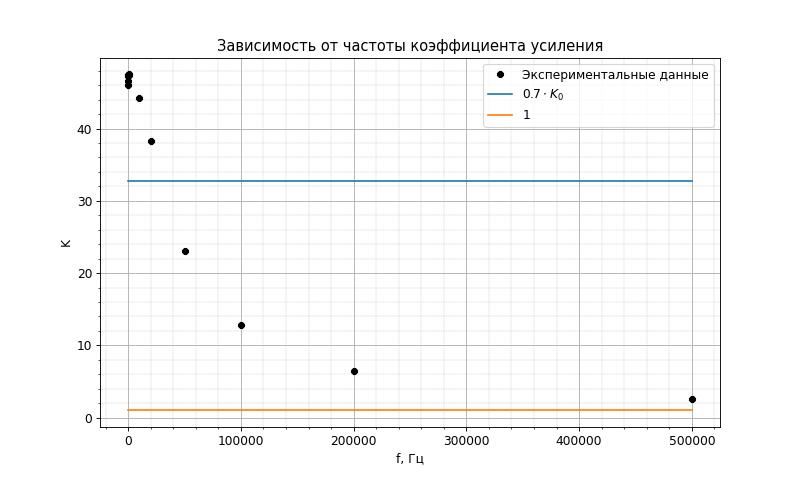
\includegraphics[width=16cm]{image2.jpg}
    \end{center}
        \caption{График зависимости относительной интенсивности от угла поворота поляроида}
        \label{img8}
    \end{figure}

    \item Провели наблюдения модовой структуры лазерного излучения. Для этого поставили на рельс вплотную к выходному зеркалу рейтер с короткофокусной линзой, за линзой поставили белый экран так, чтобы изображение было наиболее чётким. Наблюдая за пятном излучения лазера, с помощью малого поворота одного зеркала получили разные картины, описывающие разные режимы. Результаты наблюдений представлены на рисунках:
    
\end{enumerate}

\begin{figure}[h]
\begin{center}
\begin{minipage}[h]{0.48\linewidth}
    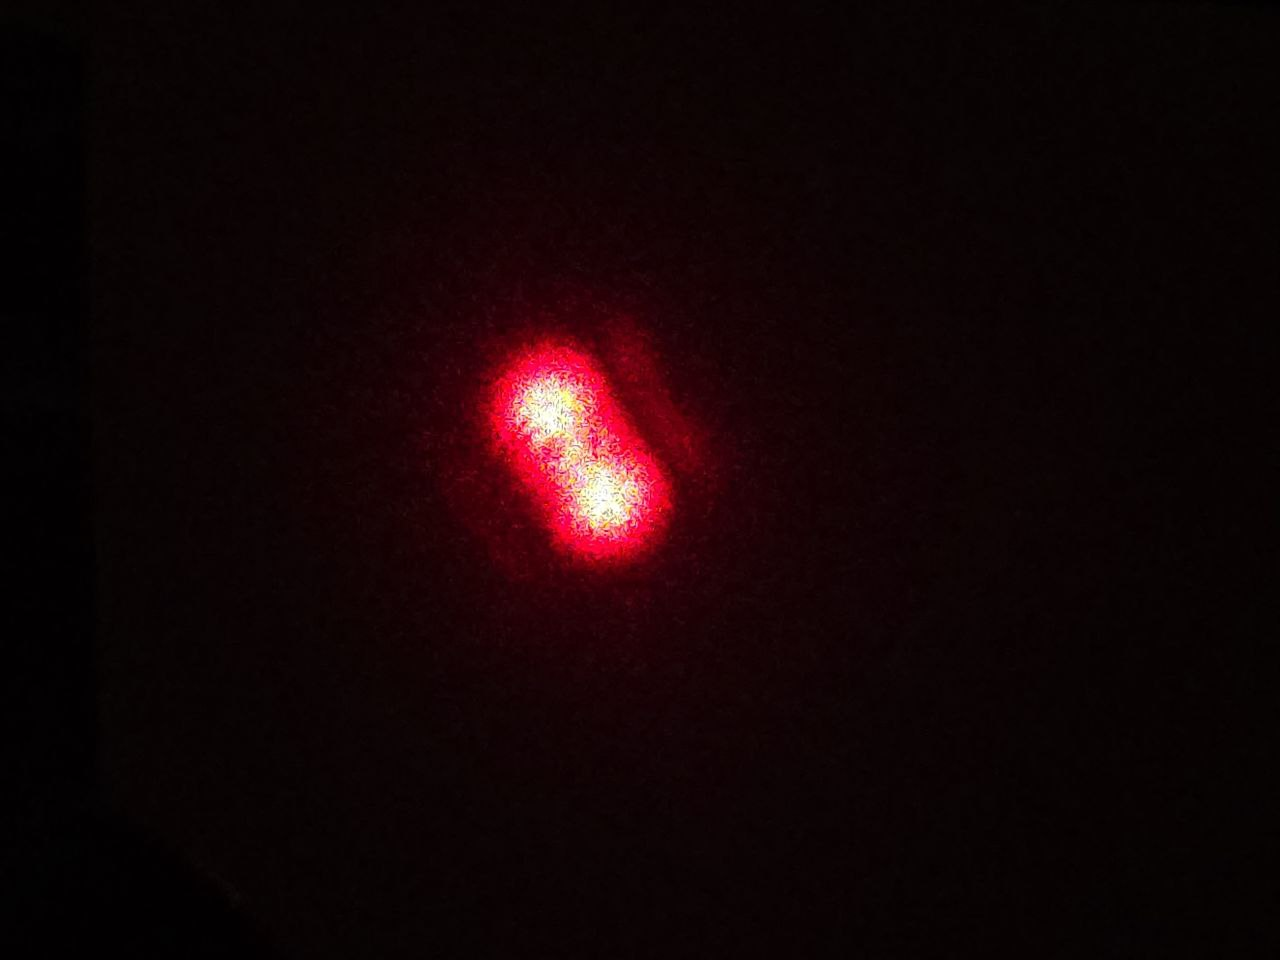
\includegraphics[width=1\linewidth]{mode2x1.jpg}
    \caption{Модовая структура 2, 1} %% подпись к рисунку
    \label{ris:experimoriginal} %% метка рисунка для ссылки на него
\end{minipage}
\hfill
\begin{minipage}[h]{0.48\linewidth}
    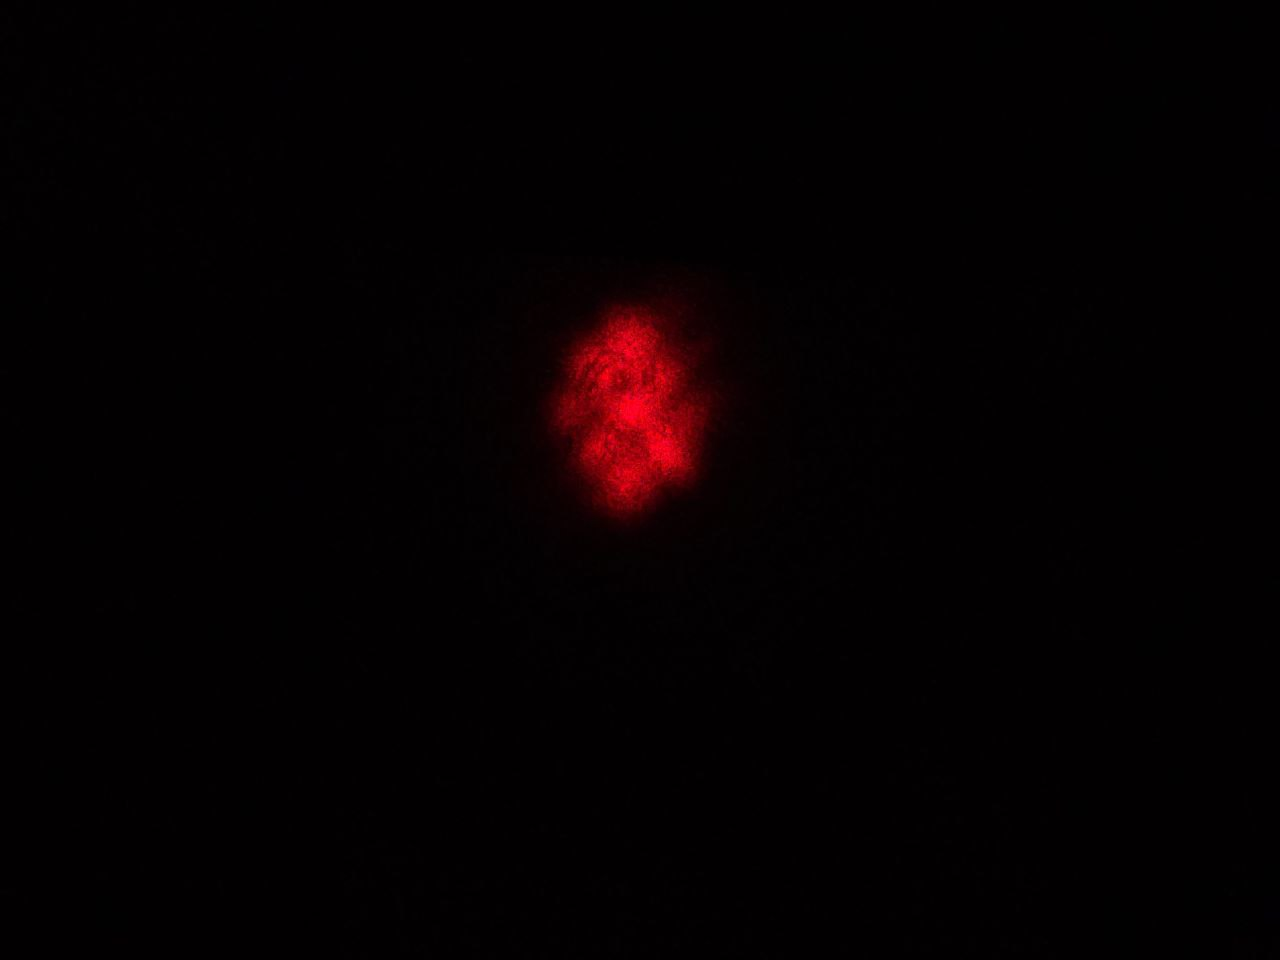
\includegraphics[width=1\linewidth]{mode2x2.jpg}
    \caption{Модовая структура 2, 2}
    \label{ris:experimcoded}
\end{minipage}
\vfill
\begin{minipage}[h]{0.48\linewidth}
    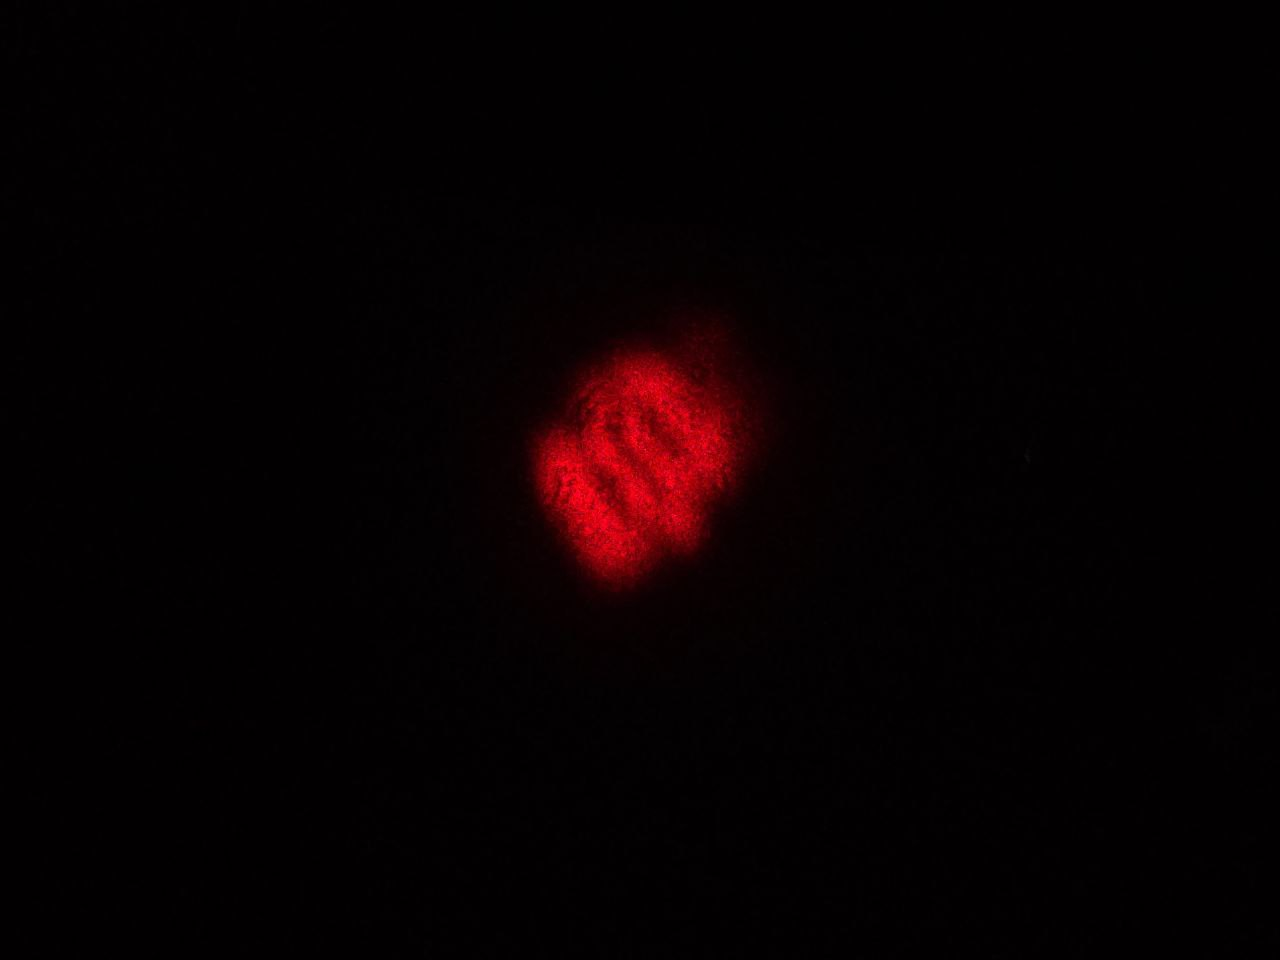
\includegraphics[width=1\linewidth]{mode3x1.jpg}
    \caption{Модовая структура 3, 1}
    \label{ris:experimcoded}
\end{minipage}
\hfill
\begin{minipage}[h]{0.48\linewidth}
    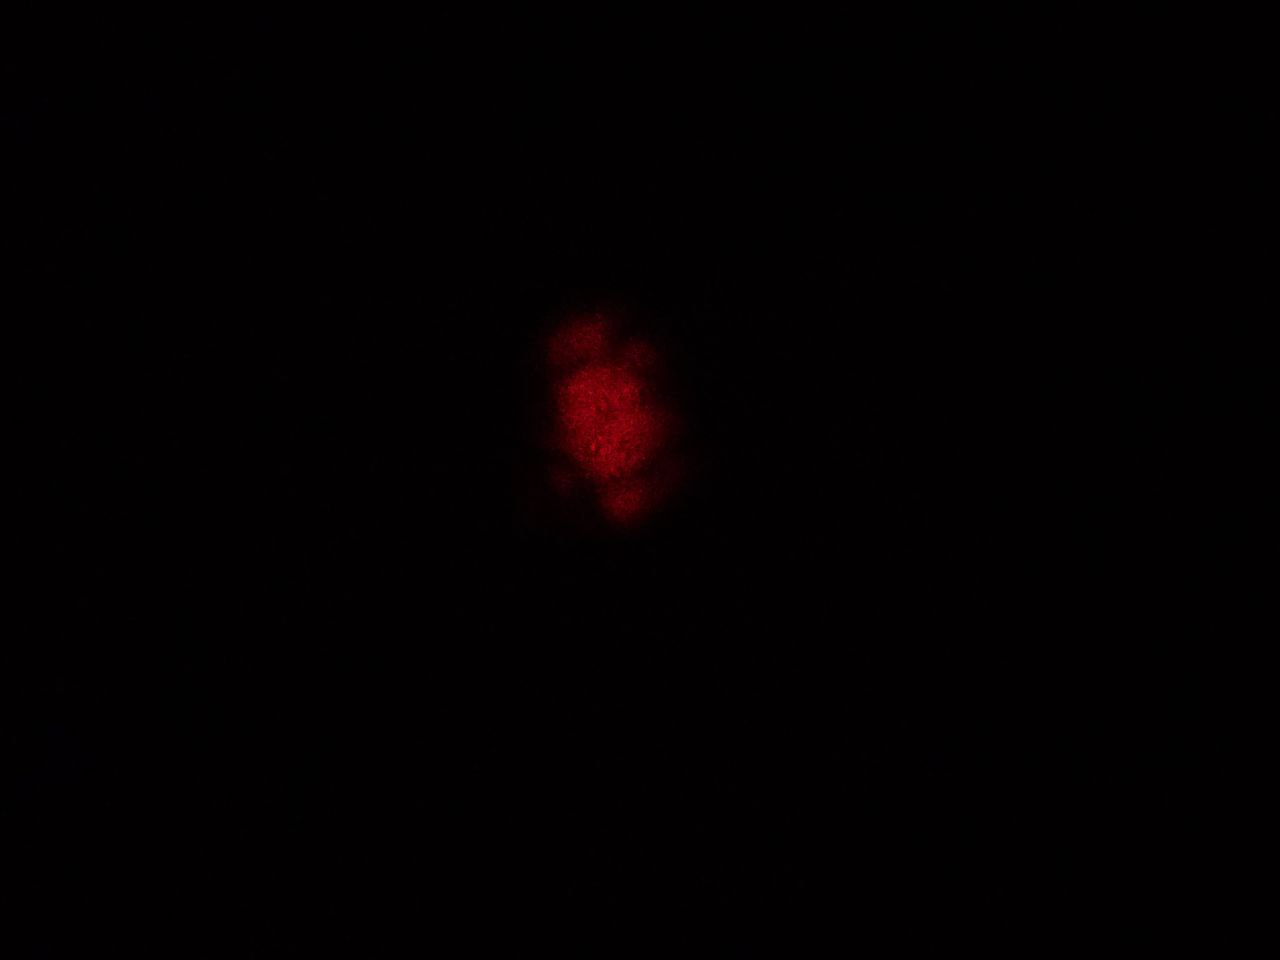
\includegraphics[width=1\linewidth]{mode3x4.jpg}
    \caption{Модовая структура 3, 4}
    \label{ris:experimcoded}
\end{minipage}
\end{center}
\end{figure}

\newpage

\section{Подведение итогов и выводы}

В ходе данной лабораторной работе мы познакомились с устройством и принципом действия гелий-неонового лазера.

Главной целью данной работы было экспериментальное измерение коэффициента усиления активной среды. К сожалению, не во всех случая нам удалось наблюдать усиление. Тем не менее, некий результат был все же достигнут.

\begin{center}
   \boxed{k=1.4\%,\text{ } \varepsilon=1.1\%} 
\end{center}

Далее мы изучили поляризацию лазерного луча и сделали вывод о том, что луч лазера линейно поляризован.

В работе также было предложено пронаблюдать поперечную модовую структуру лазерного излучения. В ходе эксперимента нам удалось увидеть режим одной моды, двух мод, а так же многомодовый режим. Характерные изображения наблюдаемых модовых режимов можно увидеть выше.

\end{document}
